\chapter{Datacollection}

\section{The need for a dataset}
To fairly compare models it is necessary for the community to have standardised datasets (REF MNIST, CIFAR ETC.). % Reference MNIST, CIFAR etc.
Many datasets exist for time-stepped models from well formatted and normalised datasets (such as MNIST) to large complex datasets (such as ***ImageNet dataset?***).
In an attempt to compare event-based processing models to time-stepped models some have tried using DVS recordings of static MNIST digits (REF O'CONOR). % ref OConor
However this doesn't capture the full potential of the DVS to capture complex spatio-temporal surfaces as the simulus is inherintly 2D.
Newer benchmark datasets have addressed this problem offering a range of stimuli, in particular complex real world self motion for a mobile robot (REF AMY PAPER). %% Ref Amy
There is still a deficency of extremely simple datasets around which strong mathmatical foundations can be laid to allow a deep understanding of network dynamics. 
As capturing movement is a key advantage of the DVS over time-stepped models this should be emphasised in the dataset. 
%This work offers such a dataset consisting of dots moving linearly with constant velocity. 

\section{Requirements and details for 8AD and AAD}
The motivations behind such a dataset must be carefully considered so when collected it forms a comprehensive set.
Simple structure is required so that when experimenting with new appraoches to processing dynamics in the system can be reasoned about with some accuracy.
Additionally a dataset for complex real world (robotic self-motion) or interesting patterns already exists, it is simpler data that is necessary.
To evaluate the accuracy of classification systems a ground truth is also required labelling events as signal or noise. 
With the advent of deep learning the advantages of large bodies of labeled training data have become apparent. 
Thus the ability to collect a large number of samples is also deemed necessary and the system should be as autonomous as possible. \\ 
\textbf{Final requirements:}

\begin{itemize}
    \itemsep-0.5em
    \item \textbf{Simplicity} -- To allow model analysis 
    \item \textbf{Movement} -- Key advantage of the DVS
    \item \textbf{Labels} -- To facilitate learning and validation
    \item \textbf{Autonomous} -- So large amounts can be captured
\end{itemize}

Considering the gap this dataset will fill and the requirements specified the simplest datum was decided to be a single dot moving linearly with a constant velocity. 
The variables to be manipulated include the dot diameter, velocity and direction. 
These variations recorded are listed in table \ref{tb:datasetspecs}.
As a stepping stone from simple datasets to more complex real world datasets two further variations were considered; two dots intersecting at the center of the screen and multiple dots tracing arbitrary angles (occationally intersecting).  

\begin{table}[h]
\centering
\begin{tabular}{ | c | l | }
    \hline
    Dot size (pixels) & 4, 6, 8 \\
    Angles (degrees) & [0 - 360] \\
    Starting position & Random \\
    Velocity (pixels/update) & 2, 4, 6, 8 \\
    \hline
\end{tabular}
\caption{Arbitrary Angle Dataset specification}
\label{tb:datasetspecs}
\end{table}

The above specification details what is from here on called the Arbitrary Angle Dataset (for berevity it will be referred to as AAD), that is, in this dataset the starting position of the dot does not restrict its direction.
An even simpler dataset from here on called the 8 Angle Dataset (for berevity, 8AD) is also presented in which the dot can only start from a corner of the screen or the middle of the one the edges.
The starting position of the dot also then dictates the direction the dot will move e.g. if it starts in the top left of the screen it must go to the bottom right or if it starts in the center of the top edge it must go to the center of the bottom edge.

% Okayyyy for 8AD lets run 250 of each angle 



%%%%%%%%%%%%%%%%%%%%%%%%%%%%       CONSIDERATIONS    %%%%%%%%%%%%%%%%%%%%%%%%%%%%%%%%%
\section{Considerations}
\subsection{Stimulus generators}
With clear requirements the practical generation of the dataset can be considered in detail.
The requirement for constant velocity would prove difficult to control in any real world system with forces of friction and gravity.
Such a real world system would also prove uneconomical in terms of time required to construct and, unless well automated, time required to conduct recordings. 
Recording computer simulations becomes an attracive option (particularly in regards to recording ground truths) but comes with its own negatives including screen refresh rates.
Recording from a computer screen also beings the disadvantage of non-continuous stimuli, the dot must be discretised, drawn onto pixels and thus screen pixel size forms the grid on which the stimuli is restricted. 
This issue can be mitigated when considering the much finer resolution of a screen compared to the DVS, the discretisation of the dot on a screen will have minimal effect if the dot is comprised of enough screen pixels.
The non-continuous stimuli issue can likewise be alliviated by restricting the dot movement to low velocities meaning in any given refresh of the screen the dot only moves by a small amount and thus approximates continuous movement. 


\subsection{Data quality concerns}
%Flashes on screen -> noise
%Light invariance
%Ground truth to actual recording consideration (mitigated through setup?)

The DVS's temporal resolution of \SI{15}{\micro\second} mean it should be able to detect screen refresh rates (every \SI{16}{\milli\second} on a 60Hz screen). 
It would be expected that every \SI{16}{\milli\second} there should activity across the whole sensor for a short time period. 
This does not seem to be the case with the DVS though, the same experiement run with the newer DAVIS sensor (with temporal resolution of \SI{3}{\micro\second} occationally is able to capture the screen refresh rate but even this is not consistant as show in figure \ref{fig:refreshFlashes}.

\begin{figure}
    \centering
    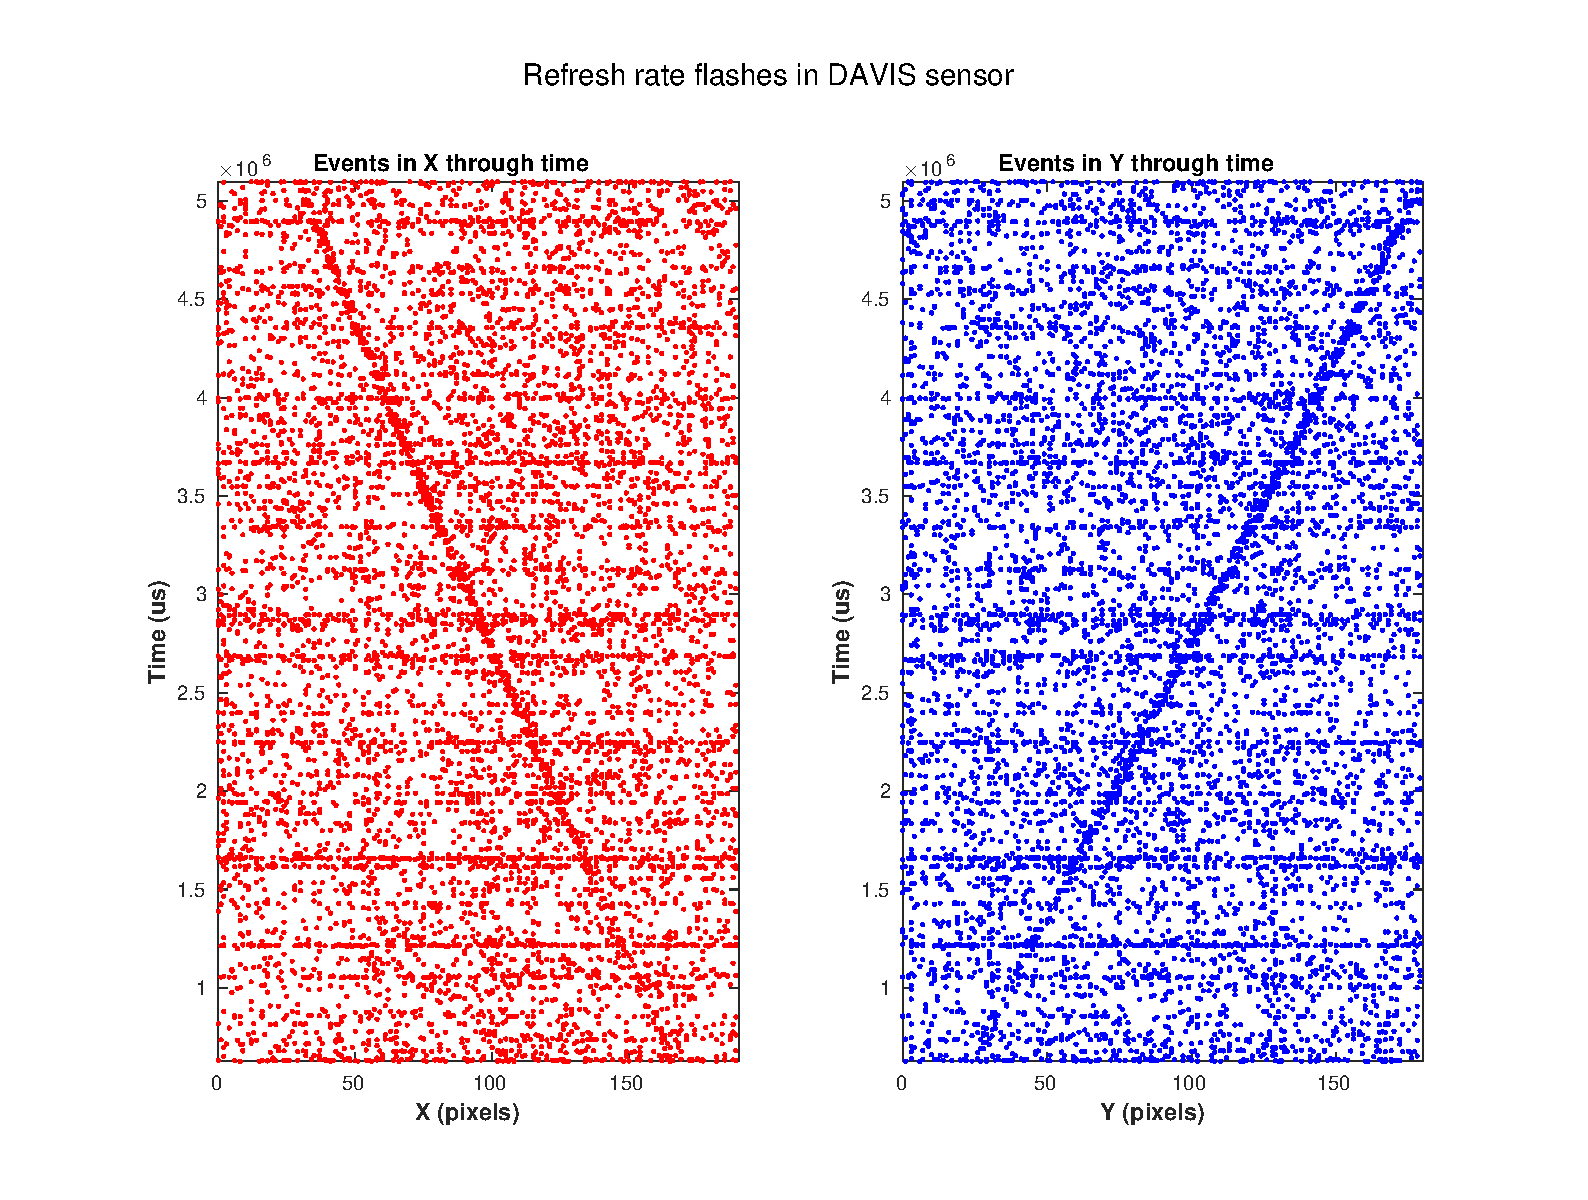
\includegraphics[width=0.8\textwidth]{screenFlashes.eps}
    \caption{Refresh rate flashes captured by DAVIS sensor}
    \label{fig:refreshFlashes}
\end{figure}

The DVS will only trigger and event if a pixels internal value has changed by 15\% meaning in low light situations the DVS will register an event more readily. 
Not all recording will be done in one session and changes to ambient light due to environmental conditions may have an impact on recording quality by triggering more or less events for the same stimuli.
This affect should be minimal if all recordings are done at roughly the same time of day in the same room with the same screen. 

A more serious concern is that of ensuring label consistency between the screen pixels and the DVS pixels. 
When recording from the screen it will be critical to ensure the DVS is carefully aligned with the edges of the stimuli.
Failure to align the two will result in labels being misleading as the recording will be offset.

\subsection{Processing considerations}
%Segmenting datasets
%Line angles (Close to edge, just a tiny segment in corner)
In an autonomous collection setup the question of data integrity must be raised.
Numerous situations could lead to the experiemental setup becoming compromised without experimenter knowledge such as the DVS being bumped.
Additionally in processing the data computer ground truth labels may accumulate an offset after many samples.
These problems can be avoided by embedding meta-data in the data recordings which keeps the processing transparent. 
The suggested meta-data to include is the trajectory of the line in this sample as well as a horizontal and vertical line crossing at the center of the screen.
This will allow callibration of the DVS's rotational and linear offset from the center of the stimulus as well as tracking of the dots path in this offset view. 
The full protocol for an experiment will thus be:

\begin{itemize}
    \itemsep-0.5em
    \item Flash dot trajectory (30\ms)
    \item Actual sample (dot following trajectory)
    \item Flash dot trajectory (30\ms)
    \item Flash cross (30\ms)
    \item Repeat for next dot and trajectory.
\end{itemize}

The process of flashing the dot trajectory, the cross and then the next dots trajectory will be referred to as a meta-flash. 
Using these meta-flashes means the data can be independently verified by other researchers and will produce a histogram of total number of spikes similar to figure *** Create and insert figure ****.
This makes segmenting samples a matter of extracting the regions in which the total number of events is below some threshold (which various proportially to the size of the dot, and hence the number of events it produces). 

%TODO figure as per figure 4 from proposal (showing use of meta-flashs).



In the arbitrary angle samples it will be possible for a dot to start close to a corner and to move to the adjacent edge resulting in a sample with a path of only a few (\textless 5) DVS pixels and lasting less than a second.
This case was considered troublesome for later processing steps and thus the starting points in the arbitrary angle dataset were restricted to the middle 80\% of each edge. 

\subsection{DVS curiosities}
%Black on white and white on black, grey
%Hot pixels

The DVS is still a new research tool and as such still has some peculiarities, in particular due to the manufacturing process some pixels, called 'hot pixels', in the array fire more frequently than others regardless of stimuli. 
These hot pixels are a source of noise in the data and could be removed in software or hardware but the effect is minimal compared with the standard noise of neuromorphic sensors so was left in these experiments. 

As mentioned when discussion lighting variations during experiments, DVS pixels will more readily fire if their internal value is smaller.
This has implications when the DVS is recording a black dot on a white screen or a white dot on a black screen.
The black screen means the DVS is more sucseptible to abient noise and will fire more events for a white dot, when compared to a black dot of the same size on a white screen. 
This phenomena is not expected to reveal any significant insight related to this thesis and is considered out of scope but its cause is worth considering whilst designing experiments. 



%%%%%%%%%%%%%%%%%%%%%%%%%%%          METHODOLOGY         %%%%%%%%%%%%%%%%%%%%%%%%%%%%%%
%TODO maybe this should just be a sub section since its so small, what else should go here?
\section{Methodology}
%What did i actually end up doing
The final system consisted of a program called dotGen written in python which would display the dot moving along a trajectory with meta-flashes.
DotGen also had tools to start a DVS recording, adjust dot parameters (size and velocity) and help set up the DVS correctly. 
DotGen would log the ground truth of the dots position to a CSV file in the format <x, y, time> every time the screen was updated.
The screen recorded from was a Dell U2414H Monitor with a refresh rate of 60Hz.
DotGen and jAER were started and the camera positioned to exactly capture the screen size then the recordings were taken. 




%%%%%%%%%%%%%%%%%%%%%%%%%%%         FINAL SPECS          %%%%%%%%%%%%%%%%%%%%%%%%%%%%%%
\section{Final dataset specifications}
Video lengths \hfill
Samples per video \hfill
Total samples \hfill
key for each filename \hfill


\section{Comments}
Looking back at the data what do i think? \hfill
Flat timestamps?? -> experimental hardware , do we still get??\hfill
% MOVE TO PROCESSING - Segmenting looses a lot on each side \hfill
%No metric for validating ground truth against actual dot accuracy
Camera angles (parallel lines not so).

The final datasets proved to be useful and to satisfy the requirements of being simple, easy to collect and of movement. 
A measure of success of the labels is harder to quantify without a metric, as the labels were not used in this work such a metric is left out of scope although this would be advantageous for the dataset. 


